%===============================================================================
% Autoři: Vladan Kudláč 2018
\chapter{Úvod}
Cílem této práce je vytvořit webovou aplikaci umožňující uživatelům upravovat videa v~internetovém prohlížeči bez nutnosti instalace dodatečných programů nebo rozšíření. Uživatel nahraje videa a obrázky ze svého zařízení nebo z~jiné služby a poté pomocí interaktivního grafického rozhraní sestříhá požadované video. Vytvořený projekt bude popsán souborem formátu XML, který zpracuje program \textit{MLT}\footnote{MLT -- sada nástrojů pro pro multimediální aplikace, \url{https://www.mltframework.org/}} na školním výpočetním clusteru. Dostupné možnosti úprav budou voleny tak, aby bylo možné editor použít pro tvorbu výukových videí. Editor bude vytvořen jako modul pro stávající projekt \textit{prednasky.com}.
Systém bude architektury klient-server. Klient bude komunikovat se serverem pomocí zdokumentovného API, aby mohla být implementace serveru nezávislá na klientu a mohli v budoucnu vzniknout různé implementace klientů. Klient bude poskytovat grafické uživatelské rozhraní pomocí HTML, CSS a Javascriptu, server bude obsluhovat požadavky, generovat XML projektů a komunikovat s~dalšími serverovými moduly. Díky této práci vznikne editor se svobodnou licencí, jako alternativa k webovým editorům s licencí ve formě předplatného a uzavřeným kódem.

Potřeby jednoduchého online video editoru vznikly při práci na portálu s výukovými videi \textit{Prednasky.com}. Při hledání řešení, které by šlo začlenit do projektu jsme zjistili, že nic takého na trhu není. Buď bylo řešení placené, nebo bylo zdarma, ale s omezenou funkčností. Ani jedno stávající řešení není s otevřeným zdrojovým kódem, které by licence dovolila použít jako komponentu projektu.

\section{Existující řešení}
Stávající řešení se dají rozdělit do dvou skupin. Desktopové video editory a online video editory. Při průzkumu existujících řešení jsem se zaměřoval zejména na projekty, které mají svobodnou licenci, nebo je lze využívat bezplatně.

\subsection{Desktopové editory}
Mezi desktopovými video editory existuje řada bezplatných řešení s~licencemi vhodnými pro další i komerční využití. Rozhraní aplikací bývá podobné, rozsáhlé, pro jednoduché editace uživatel využívá zlomek funkcí. I~v~bezplatných aplikacích lze vytvořit libovolný projekt, oproti komerčním řešení nemají žádná omezení. Nevýhodou bývá pomalá křivka učení a nutnost provozovat aplikaci na dostatečně výkoném zařízení. Z~řešení s~otevřeným zdrojovým kódem lze vyjmenovat například projekty \textit{Shotcut}\footnote{Shotcut -- bezplatný nelineární multiplatformní editor s~otevřeným zdrojovým kódem,\\\url{https://www.shotcut.org/}} a \textit{Kdenlive}\footnote{Kdenlive -- bezplatný nelineární editor pro prostředí KDE4, \url{https://kdenlive.org/}}, které používají jako jádro framework MLT.
\begin{figure}[ht]
	\centering
	\scalebox{0.6}{
		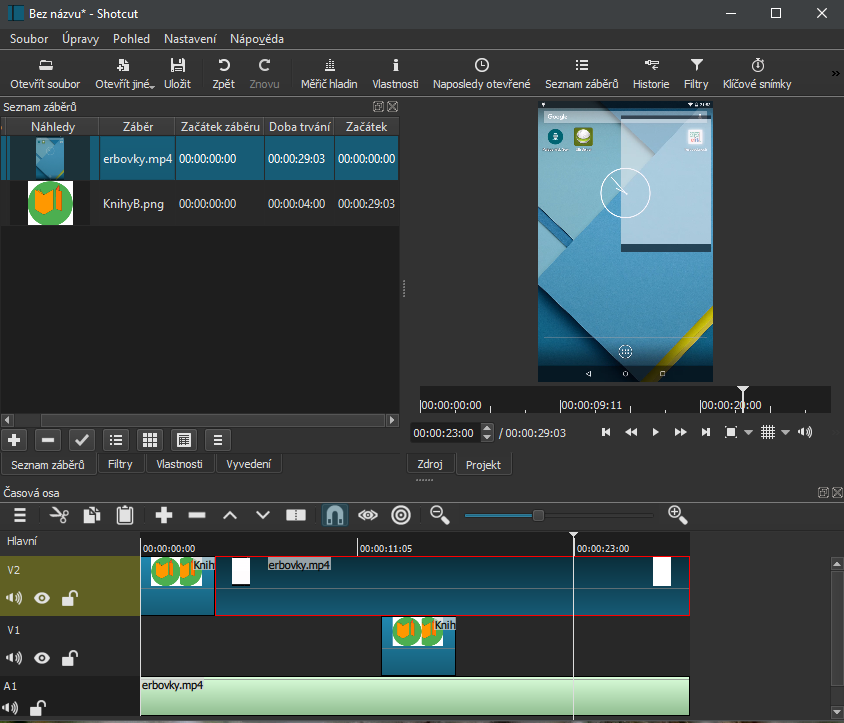
\includegraphics{obrazky-figures/shotcup.png}
	}
	\caption{Uživatelské rozhraní nelineárního video editoru Shotcut. }\label{img:shotcut}
\end{figure}
Mezi bezplatné aplikace nevyužívající framework MLT patří program \textit{Openshot}\footnote{Openshot -- bezplatný nelineární editor s~prostředím GTK+, \url{https://www.openshot.org/}}, který přešel na vlastní jádro. Mezi kvalitní proprietární programy se řadí program \textit{iMovie} od firmy Apple, \textit{Adobe Premiere Pro} od firmy Adobe Systems a \textit{ VEGAS Movie Studio} od firmy Sony. Profesionální programy se od bezplatných liší zejména vyšší stabilitou, propracovanějšími filtry a šablonami. Licence se pohybují v~řádech tisícikorun a například Adobe nabízí svůj produkt pouze ve formě předplatného.

Zajímavým projektem mezi desktopovými aplikacemi je editor \textit{fwf}\footnote{fwf -- JavaScriptový FFmpeg editor, \url{https://github.com/daem-on/fwf}.}. Jedná se o~lineární video editor využívající knihovnu FFmpeg\footnote{FFmpeg -- multiplatformní řešení pro nahrávání, konverzi a streamování audia a videa, \url{https://ffmpeg.org/}.}. Program je napsaný v~JavaScriptu a zkompilovaný pomocí nástroje Electron. Video editor nemá moc funkcí, chybí mu spolehlivost, ale lze se u~něj inspirovat s~použitými technologiemi.

\subsection{Webové editory}
U~webových editorů je velký rozdíl mezi placenými řešeními a neplacenými. Placených aplikací je nepřeberné množství s~mnoha funkcemi, bezplatná řešení mají krkolomná rozhraní a zásadní omezení. Řešení s~otevřeným zdrojovým kódem a svobodnou licencí jsem nenašel žádné.

Placena řešení se funkcemi i rozhraním blíží nativním aplikacím. Z~placených editorů zmiňuji \textit{Magisto}\footnote{Magisto -- proprietární online editor, \url{https://www.magisto.com/}.}, \textit{WeVideo}\footnote{WeVideo --  proprietární online editor, \url{https://www.wevideo.com}.}, \textit{Loopster}\footnote{Loopster -- proprietární online editor, \url{https://www.loopster.com}.} a \textit{Animatron}\footnote{Animatron -- proprietární online editor s~nejdražším předplatným, \url{https://www.animatron.com}.}. Všechny uvedené online editory mají roční předplatné, k~začátku roku 2019 se cena za nejlevnější předplatné pohybuje okolo 1341\,Kč. V~rámci nejnižšího předplatného by záznamy přednášek narážely na  maximální rozlišení výsledného videa a na maximální velikost vstupních souborů. Pro nenáročné uživatele by mohl být dostačující nástroj \textit{Clipchamp}\footnote{Clichamp -- proprietární online editor, který lze používat s~omezeními bezplatně, \url{https://clipchamp.com}.}, který nabízí i bezplatný plán s~omezením rozlišení videí na 480p.

U~bezplatných řešení jsme omezeni zejména funkcemi. Na internetu existuje řada jednoúčelových nástrojů pro úpravu videa. Komplexní video editory jsem našel dva -- \textit{Kizoa}\footnote{Kioza -- bezplatný lineární online video editor, \url{https://www.kizoa.com}.} a \textit{Movie Maker Online}\footnote{Movie Maker Online -- bezplatný online editor, \url{https://moviemakeronline.com/}.}, ani jeden není vyvíjen jako software s~otevřeným zdrojovým kódem.

Editor \textit{Kizoa} je vytvořen v~programu Adobe Flash, obsahuje dostatečné množství efektů, přechodů a nastavení. Vespod zobrazuje jednu časovou osu, jedná se o~lineární editor. Hlavní nevýhodou je vázanost na Adobe Flash Player, který je dnes na ústupu a jeho podpora skončí v~roce 2020\,\cite{FlashPlayer}.
\begin{figure}[ht]
	\centering
	\scalebox{0.53}{
		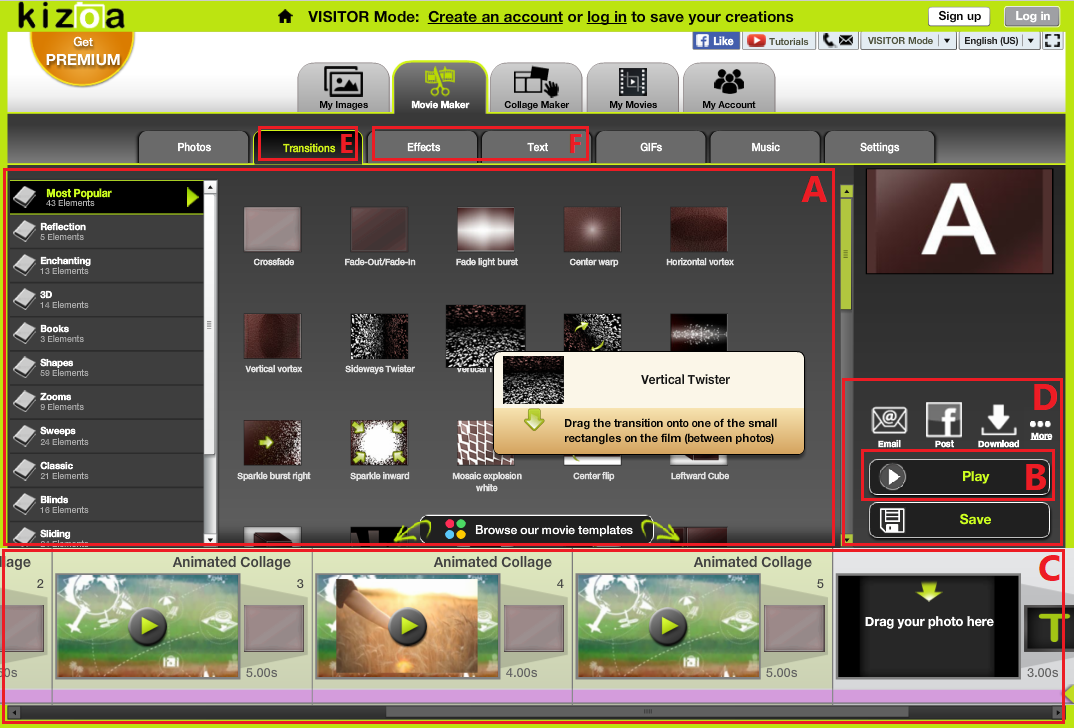
\includegraphics{obrazky-figures/kizoa.png}
	}
	\caption{Uživatelské rozhraní online lineárního video editoru Kizoa. }\label{img:kizoa}
\end{figure}

Movie Maker Online představuje video editor s~netradičním uživatelským rozhraním. Nevyužívá zásuvných modulů a osu s~videem zobrazuje vertikálně. Jedná se o~nelineární editor, který má 4 stopy -- zvukovou, stopu s~pozadím, hlavní stopu a stopu s~překryvným textem. Přidat nebo odebrat stopu není možné. Editor je řešen jako jedna stránka, na které se pod sebou nacházejí jednotlivé kroky. Nahrávání souborů probíhá v~prvním kroku, poté se musí uživatel přesunout ke kroku 2 a provést editace. Pro uživatele desktopových aplikací se jedná o~zcela jiné rozhraní, ve kterém se budou těžko orientovat. Na rozdíl od předchozího řešení neumožňuje Movie Maker Online projekt uložit nebo exportovat a později opětovně použít. 
\begin{figure}[ht]
	\centering
	\scalebox{0.53}{
		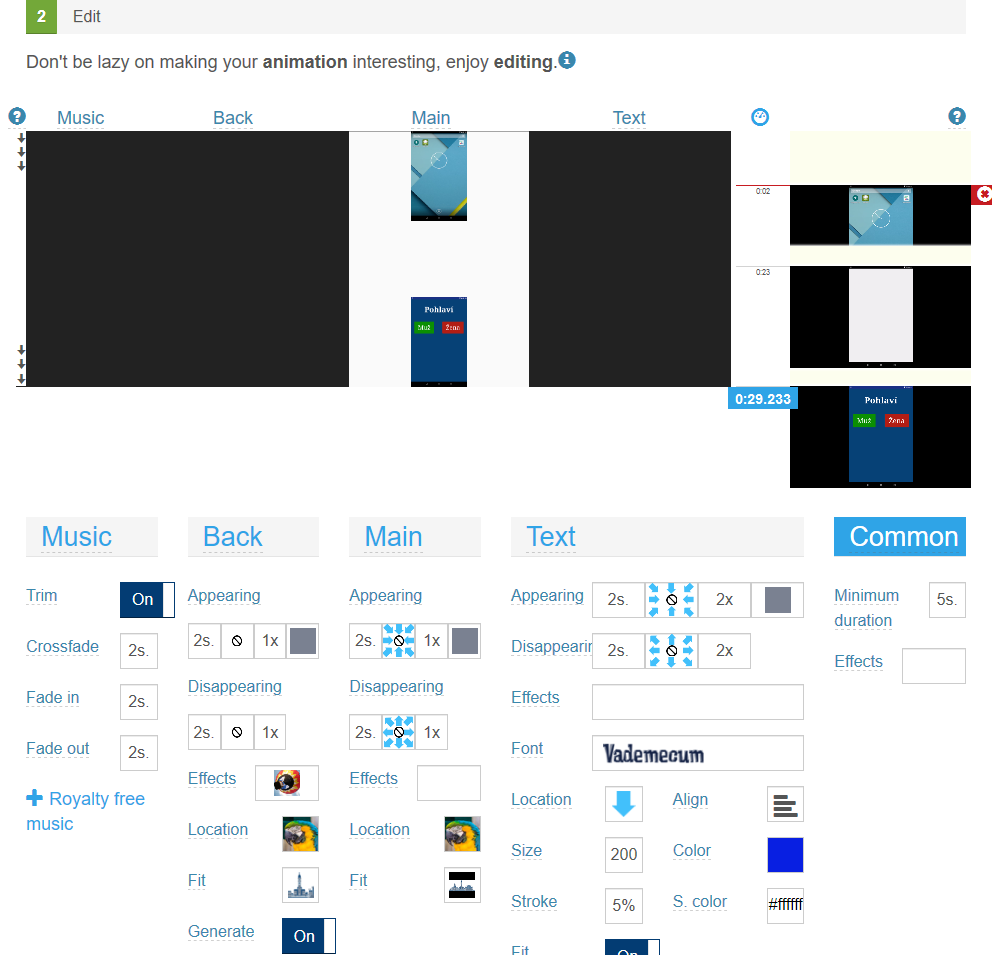
\includegraphics{obrazky-figures/moviemakeronline.png}
	}
	\caption{Uživatelské rozhraní online video editoru Movie Maker Online. }\label{img:moviemakeronline}
\end{figure}

\chapter{Teoretická část}
\section{MLT framework}
Jedná se o~sadu nástrojů s~otevřeným zdrojovým kódem s~licencí LGPL-2.1, která byla původně vytvořena pro televizní vysílání. Poskytuje nástroje pro streamování, video editory, multimediální přehrávače, konvertory a další typy multimediálních aplikací. Framework MLT umožňuje vytvářet, spravovat a přehrávat audio nebo video projekty s~více stopami. Je používán jako jako základní komponenta v~nelineárních video editorech. Využití nalezne i mimo klasické desktopové video editory, může být použit jako součást většího systému nezávisle na použitém programovacím jazyce.

Framework lze používat prostřednictvím programu \texttt{melt} v~příkazovém řádku nebo prostřednictvím MLT API knihovny v~jazyce C. Pro napojení API na jiné programovací jazyky je nutné použít \textit{SWIG}\footnote{SWIG -- nástroj pro vývoj softwaru umožňující propojit program napsaný v jazyce C/C++ s jiným jazykem, \url{http://swig.org/}.}, nástroj, který překládá volání funkcí API na volání funkcí v~C++. V~C++ funkcích se následně volají funkce programu MLT v~jazyce C. Druhou možností je provádět serializaci/deserializaci dat vlastnoručně a s~MLT komunikovat prostřednictvím formátu XML. Vnitřní struktura, kterou MLT API vytváří je XML formátu blízká. V~této práci se zabývám využitím MLT XML.

\subsection{Zprovoznění}
Framework nemá žádné jiné závislosti, než standard C99 a knihovny standardu POSIX. Zprovoznění tak zahrnuje nainstalování programu \texttt{melt} (v~případě Ubuntu z~repozitáře) a nainstalovaní programů a kodeků pro práci s~multimédii.
\begin{lstlisting}[style=bash]
$ sudo apt install melt
$ sudo apt install ladspa-sdk ffmpeg
$ sudo apt install vlc #Volitelne, pro prehrani vystupu
\end{lstlisting}

\subsection{Základní příkazy}
Jednoduché úkony lze provádět volbou parametrů při spuštění programu. Pro složitější projekty bude potřeba použít serializaci dat a formát XML. Melt umí soubory XML načítat i generovat.
\begin{lstlisting}[style=bash]
#Prehrani na obrazovce
$ melt VIDEO0004.mp4 -consumer sdl
#Predpis pro vytvoreni sedotonoveho videa serializovany v XML souboru
$ melt VIDEO0004.mp4 -filter greyscale -consumer xml > task.mlt 
#Vyvedeni souboru output.avi na zaklade XML souboru
$ melt task.mlt -consumer avformat:output.avi acodec=libmp3lame vcodec=libx264
\end{lstlisting}
\subsection{Používání formátu XML}
Nejprve je nutné uvést seznam vstupních mediálních souborů. Vstupný soubor je označen jako \texttt{producer}. U~vstupu se v~\texttt{property} uvádí hodnota \texttt{resource}, s~cestou k~souboru. Tento jednoduchý soubor po spuštění přehraje celý soubor VIDEO001.mp4. Toto XML může být užitečné pokud chceme soubor pouze překonvertovat do jiného formátu.
\begin{lstlisting}[style=xml]
<?xml version="1.0"?>
<mlt>
  <producer id="producer0">
    <property name="resource">/home/vladan/VIDEO0001.mp4</property>
  </producer>
</mlt>
\end{lstlisting}
Obvykle potřebujeme pracovat s~více soubory. K~tomuto účelu slouží \texttt{playlist}. Stanovíme vstupy (\texttt{producer}) s~unikátním \texttt{id}. V tuto chvíli by se přehrál pouze poslední soubor, který uvedeme, neboť framework MLT přehraje vždy poslední element uvnitř kořenového elementu \texttt{<mlt>} . Definujeme \texttt{playlist} obsahující položky \texttt{entry}. Vstupní soubory jsou na výstup řazeny ve stejném pořadí v~jakém jsou uvedeny v~playlistu. U~položky playlistu můžeme uvést čas (od/do) pokud chceme vložit část vstupního souboru. Časové údaje-lze zadávat buď jako počet snímků nebo jako čas ve formátu \texttt{00:00:00,000}, kde první dvojice číslic jsou hodiny a poslední tři číslice udávají milisekundy. Omezení se ignoruje, pokud uvedeme větší číslo, než je počet snímků či délka souboru. Vkládáme-li obrázek, pak hodnota \texttt{out} udá délku zobrazení obrázku. S~tímto XML zvládneme sestříhat více souborů do jednoho, vystřihnout určitou pasáž, vložit intro a outro.
\begin{lstlisting}[style=xml]
<?xml version="1.0"?>
<mlt>
  <producer id="producer0">
    <property name="resource">/home/vladan/VIDEO0004.mp4</property>
  </producer>
  <producer id="producer1">
    <property name="resource">/home/vladan/VIDEO0001.mp4</property>
  </producer>
  <producer id="producer2">
    <property name="resource">/home/vladan/lego1.png</property>
  </producer>

  <playlist id="playlist0">
    <entry producer="producer2" in="0" out="50"/>
    <entry producer="producer1" in="0" out="999"/>
    <entry producer="producer0" in="0" out="100"/>
  </playlist>
</mlt>
\end{lstlisting}
Chceme-li na video aplikovat filtry, musíme vytvořit element \texttt{tractor} obsahující \texttt{multitrack} se seznamem tracků (playlistů). V~tractoru definujeme filtry. Filtry aplikujeme na \texttt{track} (playlist). Pokud budeme chtít vzít vstupní video, aplikovat na něj černobílý filtr, musíme vytvořit \texttt{playlist} s~jedním zdrojem a \texttt{tractor} s~jedním playlistem (track).
\begin{lstlisting}[style=xml]
<?xml version="1.0"?>
<mlt>
  <producer id="producer0">
    <property name="resource">/home/vladan/VIDEO0002.mp4</property>
  </producer>
  <tractor id="tractor0">
    <multitrack>
      <playlist id="playlist0">
        <entry producer="producer0"/>
      </playlist>
    </multitrack>
    <filter mlt_service="greyscale" track="0"/>
  </tractor>
</mlt>
\end{lstlisting}
Pokud potřebujeme aplikovat filtr na část videa, musíme vytvořit dva playlisty -- jeden pro část na kterou bude aplikován filtr a druhý playlist pro část bez filtru. Pro synchronizaci playlistů použijeme \texttt{blank}, v~jednu chvíli se může zobrazovat pouze jeden z~playlistů, přednost má ten později zadefinovaný. V~následujícím případě se v~playlist1 prvních 100 snímků přehrává VIDEO0002, v~playlist2 je po tuto dobu nastaven stav \texttt{blank}. Pokud chceme zobrazovat statickou překryvnou vrstvu, můžeme využít filtru \texttt{watermark}. Pokud je filtr přizpůsobitelný parametry, uvedou se uvnitř elementu \texttt{filter} stejným způsobem, jako se uvádí parametry u elementů \texttt{producer}.
\begin{lstlisting}[style=xml]
<?xml version="1.0"?>
<mlt>
  <producer id="producer0">
    <property name="resource">/home/vladan/VIDEO0002.mp4</property>
  </producer>
  <tractor id="tractor0">
    <multitrack>
      <playlist id="playlist0">
        <entry producer="producer0" in="0" out="99"/>
        <blank length="50"/>
        <entry producer="producer0" in="150"/>
      </playlist>
      <playlist id="playlist1">
        <blank length="100"/>
        <entry producer="producer0" in="100" out="149"/>
      </playlist>
    </multitrack>
    <filter mlt_service="watermark" track="0">
      <property name="resource">transparent.png</property>
    </filter>
    <filter mlt_service="greyscale" track="1"/>
  </tractor>
</mlt>
\end{lstlisting}
Více stop (\texttt{track}) může být přehráváno současně pouze použijeme-li filtr nebo přechod. Přechody (\texttt{transition}) se aplikují stejně jako filtry uvnitř tractoru. U~přechodu nastavíme snímek náběhu a dokončení přechodu (\texttt{in} a \texttt{out}) a dále specifikujeme typ přechodu (\texttt{mlt\_service}) dle \url{https://www.mltframework.org/plugins/PluginsTransitions/}, počáteční stopu přechodu (\texttt{a\_track}) a cílovou stopu přechodu (\texttt{b\_track}). Tímto způsobem můžeme vytvořit intro nebo outro s~přechody, či prolínání jednotlivých video souborů. Obě stopy by se měly překrývat pouze po dobu přechodu. Pokud by například přechod skončil dříve, než by začala druhá stopa, docházelo by ke krátkodobému probliknutí první stopy.
\begin{lstlisting}[style=xml]
<mlt>
  <producer id="producer0">
    <property name="resource">lego1.png</property>
  </producer>
  <producer id="producer1">
    <property name="resource">VIDEO0001.mp4</property>
  </producer>
  <tractor id="tractor0">
    <multitrack id="multitrack0">
      <playlist id="playlist0">
        <entry producer="producer0" in="0" out="74"/>
      </playlist>
      <playlist id="playlist1">
        <blank length="50"/>
        <entry producer="producer1"/>
      </playlist>
    </multitrack>
    <transition mlt_service="luma" in="50" out="74" a_track="0" b_track="1"/>
  </tractor>
</mlt>
\end{lstlisting}

S~pomocí těchto konstrukcí jsme schopni nadefinovat nejčastější operace, které se při zpracovávání přednášek provádí.

\section{Manipulace s videi v prohlížeči}
S příchodem HTML5 prvků \texttt{<video>} a \texttt{<audio>} a jejich JavaScriptového API vzniká možnost práce s multimédií na webu. Práci s multimediálními prvky implementovali od roku 2010 všechny moderní prohlížeče. Za moderní desktopové prohlížeče považuji program Google Chrome, Safari, Mozilla Firefox, Opera, Microsoft Edge. Prohlížeč Internet Explorer má sice dle serveru StatCounter\footnote{StatCounter Global Stats -- statistiky zastoupení prohlížečů, \url{http://gs.statcounter.com/browser-market-share/desktop/worldwide/#monthly-201803-201903}.} 5.48\% zastoupení, což jej řadí mezi Microsoft Edge a Operu, avšak i zaměstnanec Microsoftu jej v únoru označil za \uv{řešení pro kompatibilitu}, nikoliv webový prohlížeč.\footnote{Nebezpečí používání Internet Explorer jako výchozího prohlížeče, \url{https://techcommunity.microsoft.com/t5/Windows-IT-Pro-Blog/The-perils-of-using-Internet-Explorer-as-your-default-browser/ba-p/331732}.} Internet Explorer získává bezpečnostní záplaty, ale neprobíhá implementace nových webových standardů. Při vývoji nových projektů by tedy nekompatibilita s Internet Explorer neměla být brána v potaz.

\subsection{Kódování}
Veškerá data v počítači je potřeba kódovat. Na vyšší úrovni pohlížíme na kódování jako na formát dat. Formáty kódování audia  jsou například MP3, AAC, Vorbis, FLAC a formáty kódování videa například MPEG-2, MPEG-4 , H.264, HEVC, Theora, VP9, AV1.  Z pohledu uživatele se liší zejména licencí pro použití a způsobem komprese dat. Multimediální soubory mohou obsahovat více video a audio stop, titulky či jiná podpůrná data, proto se multimediální soubory vždy obalují do multimediálních kontejnerů, jako například AVI, MP4, FLV, RealMedia, Matroška. Výběr formátu videa tak typicky zahrnuje výběr multimediálního kontejneru, formátu kódování videa a formátu kódování audia. Kodek je zařízení nebo počítačový program, který dokáže převádět zakódovaná data do jiné podoby, v případě webových aplikací je kodekem internetový prohlížeč. V době, kdy organizace W3C\footnote{World Wide Web Consortium (W3C) -- mezinárodní sdružení vytvářející webové standardy, \url{https://www.w3.org/}.} vytvářela specifikaci pro HTML5 prvky \texttt{<video>} a \texttt{<audio>} byla snaha standardizovat formát, který by byl podporován ve všech prohlížečích neúspěšná kvůli požadavku na royalty free licenci.\cite{HTML5multimedia} Od té doby se nejvíce rozšířil formát MP4 H.264, který ovšem odmítá Mozilla a Theora, který odmítá Apple. Pokud se podíváme dnes na srovnání podporovaných kodeků, tabulka \ref{tab:codecs}, zjistíme, že situace není jednoduchá.
\begin{table}[h]
    \centering
    \begin{tabular}{|l|l|l||l|l|l|l|l|}
    \hline
    Kontejner   & Video & Audio & Chrome & Firefox & Edge & Opera & Safari \\
    \hline
    WebM        & VP8   & Vorbis &ano & ano & s 2 rozšířeními & ano & ne* \\
    WebM        & VP9   & Opus & ano & ano & rozšíření, HW dekodér & ano & ne \\
    WebM        & AV1   & Opus/Vorbis & ano & ano & s beta rozšířením & ano & ne \\
    Ogg         & Theora & Vorbis & ano & ano & s rozšířením & ano & ne \\
    MP4         & H.264 & MP3 & ano*** & ano** & ano & ano & ano \\
    MP4         & H.264 & AAC & ano*** & ano** & ano & ano & ano \\
    \hline
    \end{tabular}
    \caption{Přehled nejčastěji podporovaných formátů videa internetovými prohlížeči.}
    \label{tab:codecs}
\end{table}\\
* Safari vyžaduje pro VP8 program Perian\footnote{Perian -- program pro MacOS rozšiřující podporu QuickTime o další formáty (vývoj ukončen) ,\url{https://www.perian.org/}.}.\\
** Mozilla Firefox pro Linux vyžaduje pro H.264 program GStreamer\footnote{GStreamer -- otevřený multiplatformní multimediální framework, \url{https://gstreamer.freedesktop.org/}.} nebo FFmpeg.\\
*** Google Chrome H.264 podporuje, ale Chromium vyžaduje FFmpeg.
\medskip

Pokud bychom chěli použít pouze jeden formát, můžeme zvolit H.264 video s AAC audiem uvnitř MP4 nebo VP8 video s Vorbis audiem uvnitř WebM. V prvním případě budou muset uživatelé prohlížeče Firefox na Linuxových systémech a uživatelé prohlížeče Chromium nainstalovat program FFmpeg, v druhém případě budou muset užiatelé Safari nainstalovat program Perian a uživatelé Microsoft Edge Rožšíření pro webová média a Rozšíření pro video VP9. Chceme-li mít jistotu, že uživatel video přehraje, pak musíme zvolit formáty dva -- H.264 s MP3/AAC uvnitř MP4 pro uživatele Safari a Edge a pro ostatní uživatele variantu Theora s Vorbis uvnitř Ogg.
\chapter{Návrh řešení}
\section{Požadavky na řešení}
Operace nad videi jsou členěny do několika částí, pro větší přehlednost uvádím diagram případů užití pro každou část zvlášť.

V~seznamu zdrojů je možné nahrávat obrázkové a video soubory. Podporované formáty video souborů jsou shodné s~formáty, které podporuje multimediální framework FFmpeg. Z~obrázkových souborů je podporován formát PNG a JPEG, obrázek \ref{img:ucd-zdroj}.
% [Uživatel]-(Nahrát video nebo obrázek),
% [Uživatel]-(Odebrat video nebo obrázek),
% [Uživatel]-(Vložit video na konec časové osy),
% [Uživatel]-(Vložit obrázek na konec časové osy),
% (Vložit obrázek na konec časové osy)>(Nastavit dobu trvání),
\begin{figure}[h]
	\centering
	\scalebox{0.4}{
		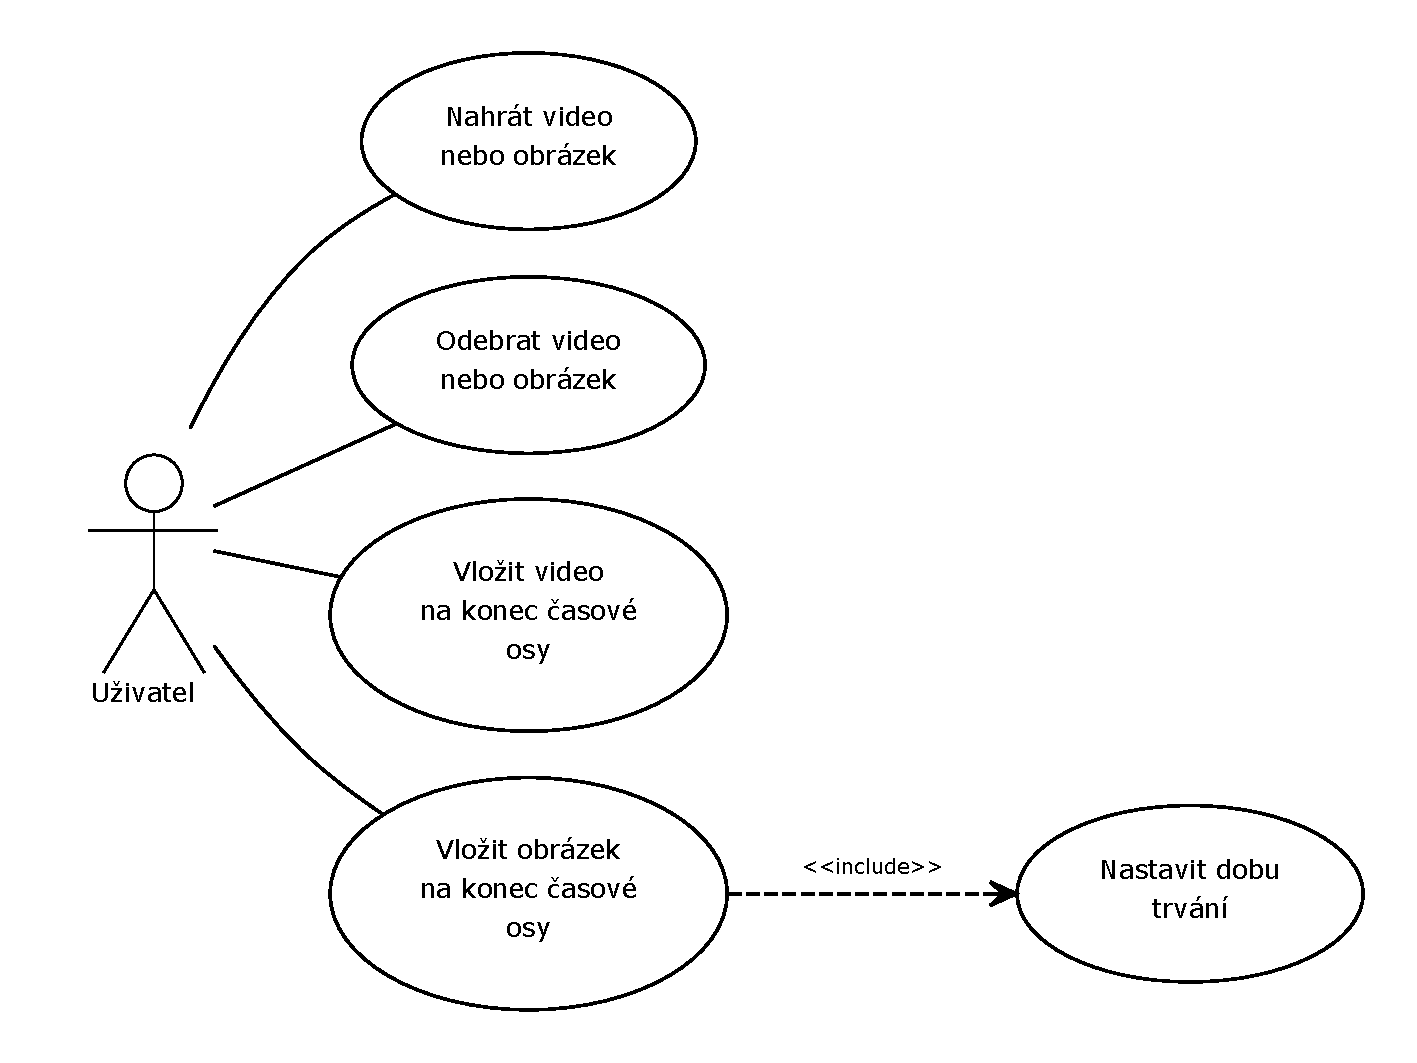
\includegraphics{obrazky-figures/ucd-zdroje.pdf}
	}
	\caption{Diagram případů užití pro práci se zdroji.}\label{img:ucd-zdroj}
\end{figure}

Časovou osu lze přibližovat a oddalovat tlačítky v~liště nástrojů časové osy. Pokud je časová osa přiblížena natolik, že není možné zobrazit všechny prvky časové osy, lze osu posouvat do stran uchopením prázdného místa na ose a přetažením osy do stran. V~novém projektu je k~dispozici jedna časová a jedna zvuková stopa. V~případě potřeby lze přidat novou stopu tlačítkem z~lišty nástrojů časové osy. K~dispozici je buď zvuková nebo video stopa. Odebrat ji lze tlačítkem vlevo pod názvem stopy. Kliknutím do prostoru časových hodnot osy se provede přemístění ukazatele aktuálního času, ukazatel lze rovněž uchopit a přesunout. V~čase ukazatele se bude přehrávat náhled videa a v~tomto čase lze provést střih videa, obrázek \ref{img:ucd-osa}.
% [Uživatel]-(Přiblížit časovou osu),
% [Uživatel]-(Posunout časovou osu do stran),
% [Uživatel]-(Přidat nebo odebrat časovou osu),
% [Uživatel]-(Nastavit pozici ukazatele)
\begin{figure}[h]
	\centering
	\scalebox{0.4}{
		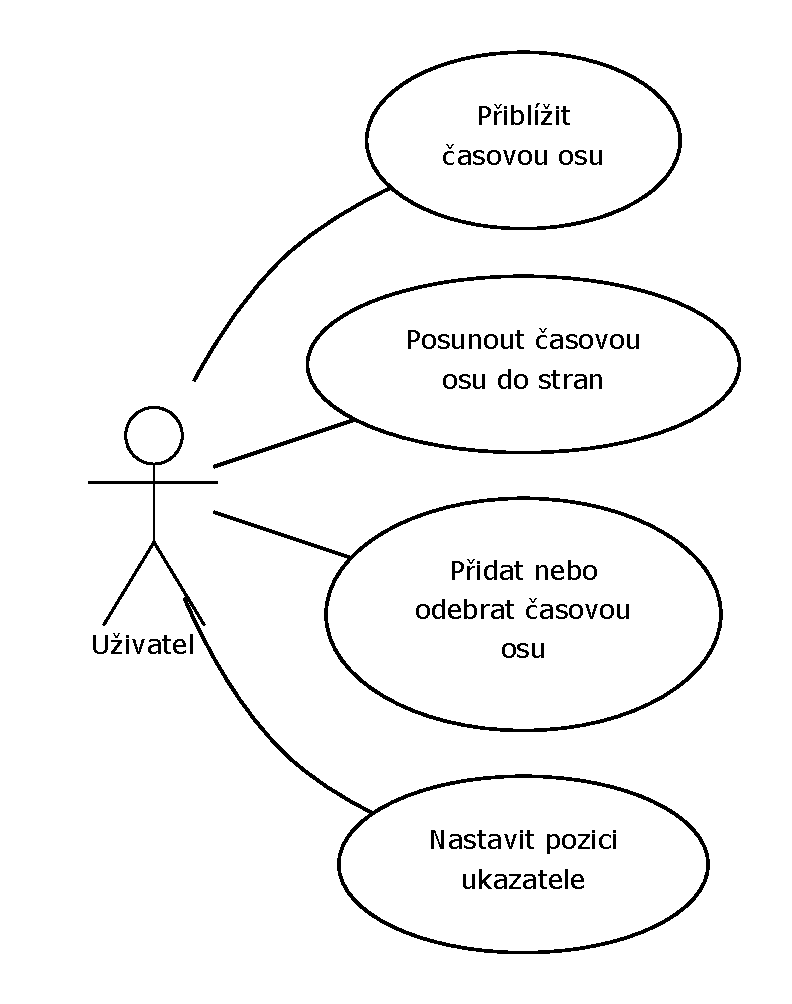
\includegraphics{obrazky-figures/ucd-osa.pdf}
	}
	\caption{Diagram případů užití pro práci s~časovou osou.}\label{img:ucd-osa}
\end{figure}

Po vybrání položky (videa nebo obrázku) na časové ose jsou k~dispozici v~panelu nástrojů časové osy následující akce. Položku lze smazat, okolní položky zůstávají, přechody se zruší. Lze přidat filtr obrazu (text, HTML překrytí, jas, kontrast, odstín, světlost, sytost, vyvážení bílé, otočit, velikost, poloha, ořezání, průhlednost, ostrost) nebo filtr zvuku (ztišit, zesílit/zeslabit). Přidat přechod mezi 2 položkami, položky s~přechody se při přesouvání chovají jako celek. Dále lze zobrazit souhrnné vlastnosti. Následující úkony se neprovádí přes panel nástrojů -- posun na časové ose se provede uchopením prvku a přetažením na nové místo, přesun na jinou časovou se provádí přetažením na jinou osu stejného typu a začátek nebo konec video souboru či délku obrázku lze změnit uchopením okraje položky a táhnutím na požadovanou pozici. Rozdělení v~bodě na 2 části se provede v~místě, na kterém je ukazatel časové osy, obrázek \ref{img:ucd-polozky}.
% [Uživatel]-(Posunout na časové ose),
% [Uživatel]-(Přesunout na jinou časovou osu),
% [Uživatel]-(Vybrat pro práci),
% [Uživatel]-(Změnit začátek nebo konec ořezem),
% [Uživatel]-(Rozdělit v bodě na 2 části),
% (Vybrat pro práci)<(Odstranit z časové osy),
% (Vybrat pro práci)<(Přidat filtr),
% (Vybrat pro práci)<(Přidat přechod mezi 2 položkami),
% (Vybrat pro práci)<(Zobrazit vlastnosti),
\begin{figure}[!h]
	\centering
	\scalebox{0.4}{
		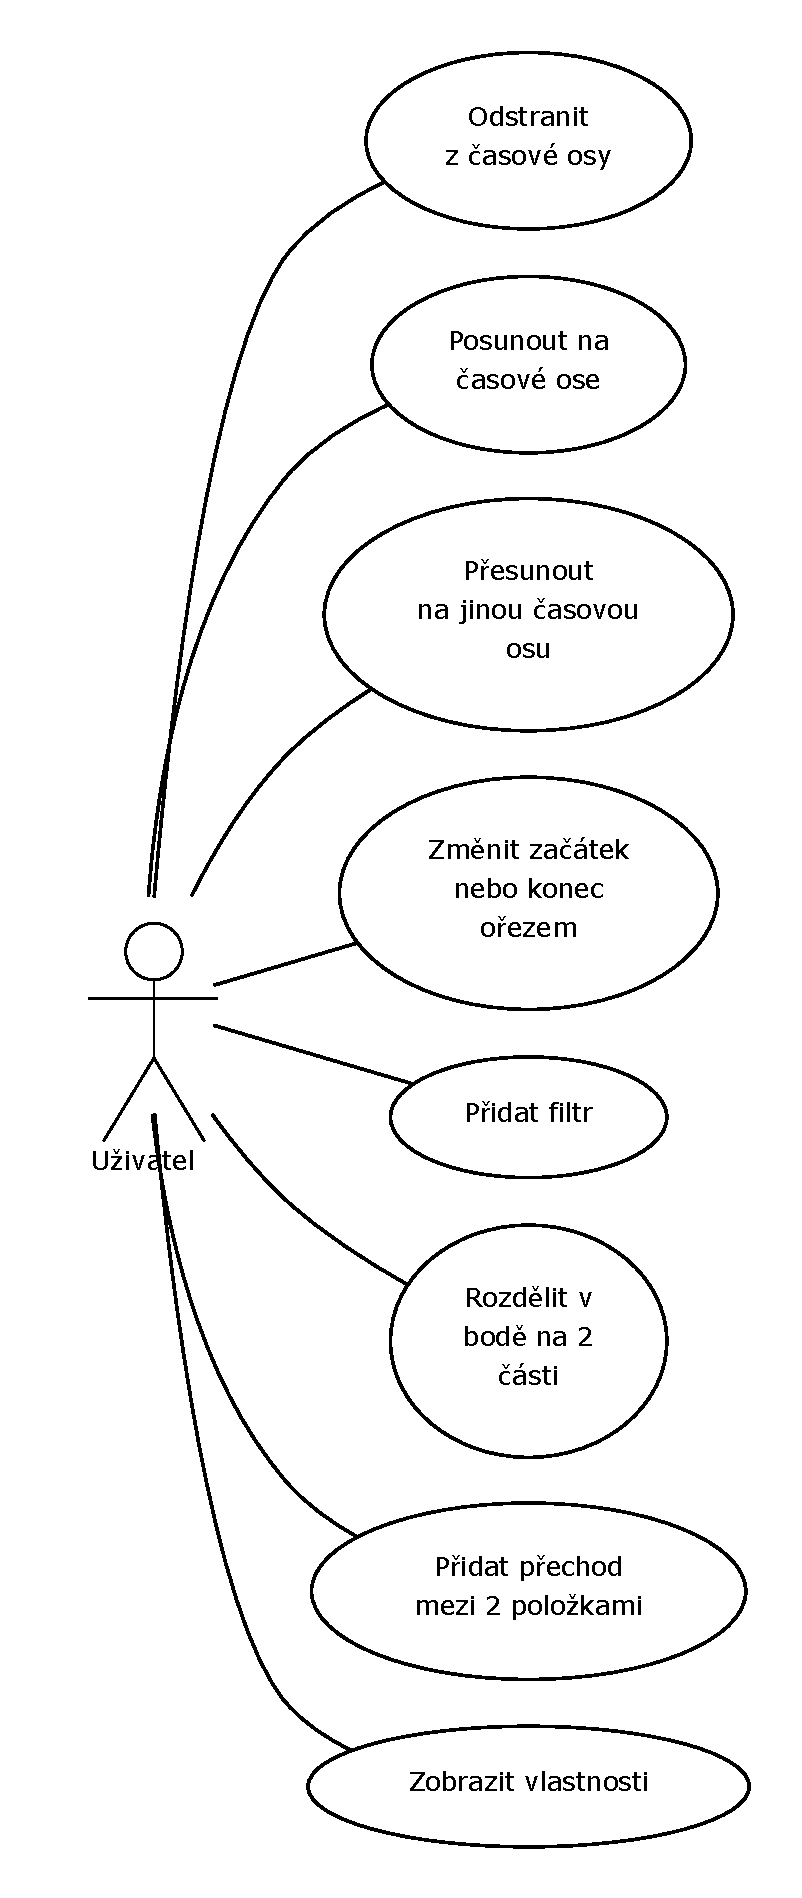
\includegraphics{obrazky-figures/ucd-polozky.pdf}
	}
	\caption{Diagram případů užití pro práci s~položkami časové osy.}\label{img:ucd-polozky}
\end{figure}

V~pravé polovině se nachází přehrávač náhledu, ovládá se tlačítky pod přehrávačem. Aktuální pozici přehrávače udává ukazatel na časové ose. Přehrávání lze spustit původní rychlostí a pozastavit. K~manipulaci s~pozicí ve videu slouží skok na událost vpřed/vzad, který přesune ukazatel na nejbližší začátek nebo konec položky libovolné stopy. Pro nejjemnější doladění slouží skok na další/předchozí snímek, obrázek \ref{img:ucd-prehravac}.
% [Uživatel]-(Spustit přehrávání),
% [Uživatel]-(Pozastavit přehrávání),
% [Uživatel]-(Skok na událost vpřed nebo vzad),
% [Uživatel]-(Další nebo předchozí snímek),
\begin{figure}[!h]
	\centering
	\scalebox{0.4}{
		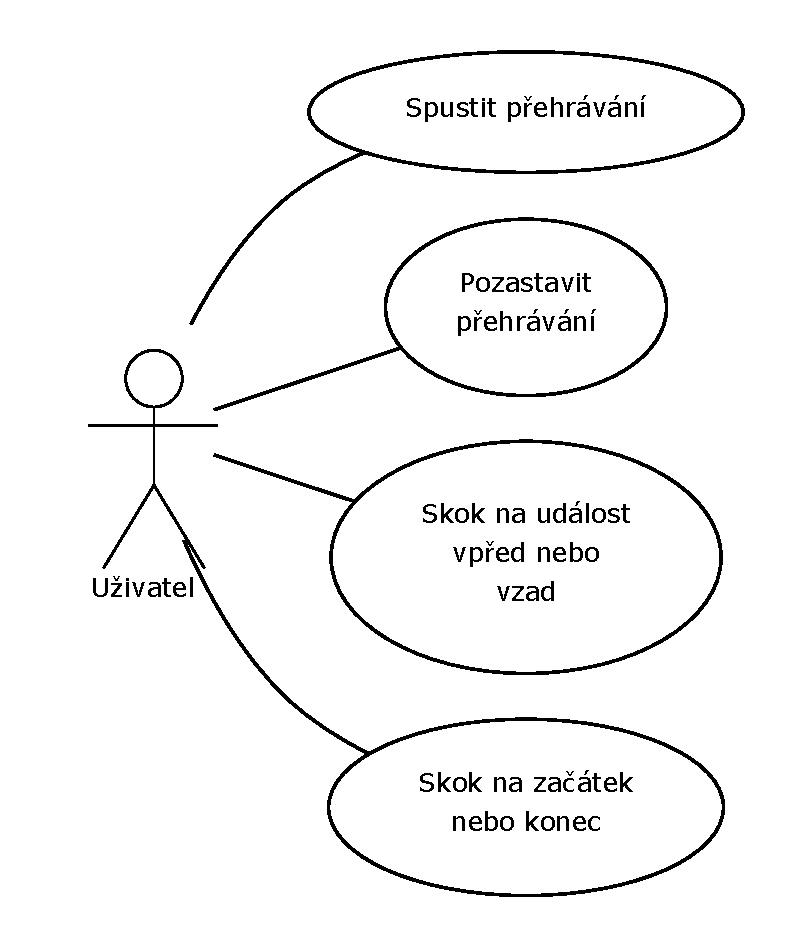
\includegraphics{obrazky-figures/ucd-prehravac.pdf}
	}
	\caption{Diagram případů užití pro práci s~přehrávačem náhledu.}\label{img:ucd-prehravac}
\end{figure}

Pokud má nový systém nahradit stávájící proces zpracování videa, musí zvládat všechny kroky úprav videa. V~Tabulce \ref{tab:uc1} uvádím v~současnosti nejčastější případ užití, kdy je potřeba oříznout začátek a konec videa a před video vložit úvodní obrazovku s~podmínkami použití.

\begin{table}[h]
    \centering
    \begin{tabular}{|p{14cm}|}
        \hline
        Případ užití: Vložit intro, oříznout videozáznam\\ \hline
        \textbf{ID: UC1}\\ \hline
        \textbf{Účastníci:}\\
        Zaměstnanec FIT\\
        Systém\\ \hline
        \textbf{Vstupní podmínky:}\\
        1. Zaměstnanec má k~dispozici obrázek s~intro a video.\\
        2. Zaměstnanec otevřel internetové stránky s~editorem.\\ \hline
        \textbf{Tok událostí:}\\
        1. Případ užití začíná nahráním videa a obrázku intra.\\
        2. Uživatel vloží obrázek na časovou osu, v~dialogu nastaví délku zobrazení intra.\\
        3. Uživatel vloží video na časovou osu.\\
        4. Uživatel si přehraje náhled videa a v~místě plánovaného začátku a konce videa přehrávání pozastaví a provede rozdělení na 2 části.\\
        5. Uživatel zvolí část po plánovaném konci a odstraní ji.\\
        6. Uživatel zvolí část před plánovaným začátkem a odstraní ji. Ořezané video uchopí a přetáhne jej na časové ose hned za konec intra.\\
        7. Uživatel potvrdí změny a vyplní parametry výsledného videa.\\
        8. Systém generuje XML a nabízí jej ke stažení nebo zpracování na serveru.\\
        \hline
    \end{tabular}
    \caption{Textová specifikace případů užití pro nejčastější úpravy záznamů přednášek.}
    \label{tab:uc1}
\end{table}

\section{Uživatelské rozhraní}
Při návrhu uživatelského rozhraní jsem se nejvíce inspiroval desktopovou aplikací \textit{Shotcut} a online nástrojem pro úpravu fotografií -- \textit{Photopea}\footnote{Photopea.com -- bezplatný editor fotografií, \url{https://www.photopea.com/}}.

Uživatelské rozhraní je rozděleno do 3 částí. V~levé části se nachází seznam zdrojového materiálu (videí, obrázků, aj.), který je možné v~projektu použít. V~pravé části se nachází přehrávač předběžného náhledu výsledného videa. Ve spodní části je časová osa se zvukovými a obrazovými stopami. Rozložení bylo navrženo drátěným modelem, obrázek \ref{img:wireframe}.

\begin{figure}[h]
	\centering
	\scalebox{0.3}{
		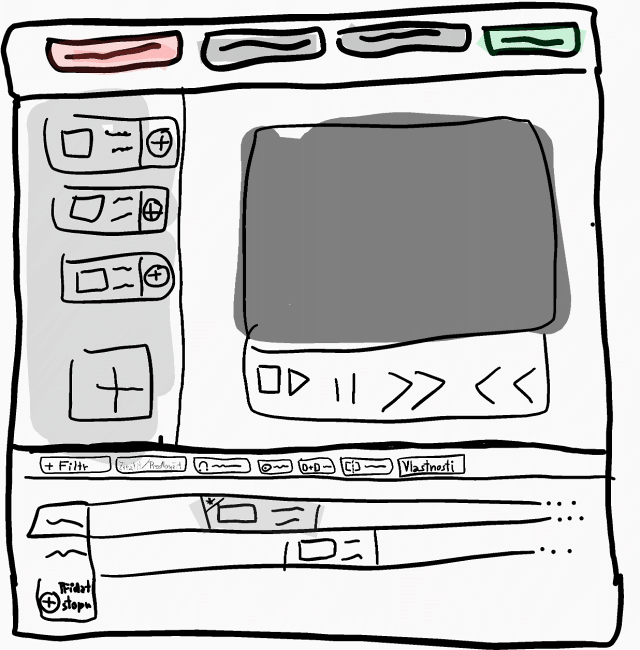
\includegraphics{obrazky-figures/wireframe}
	}
	\caption{Drátěný model uživatelského rozhraní.}\label{img:wireframe}
\end{figure}

Globální akce, jako například zrušení či dokončení projektu, export projektu, jsou prováděny v~panelu nástrojů u~horního okraje obrazovky.

Přehrávač náhledu se ovládá tlačítky umístěnými přímo pod přehrávačem (přehrát, zastavit, posun o~snímek, skok na začátek nebo konec). Přehrávač přehrává pouze soubory umístěné na časové ose, nezobrazuje náhledy zdrojového materiálu.

S~položkami seznamu se zdrojovým materiálem se pracuje přímo. Po najetí nebo kliknutí na položku se zobrazí dostupné operace. Pod poslední položkou se nachází tlačítko na přidání materiálu, případně je možné použít přetažení souboru do oblasti seznamu.

Časová osa zobrazuje pod sebou stopy v~pořadí, v~jakém byly přidány. Stopu lze odebrat či přidat novou zvukovou nebo obrazovou stopu tlačítkem pod poslední stopou. Položky se na časovou osu přidávají přetažením ze seznamu materiálu a nebo tlačítkem plus u~materiálu. Poloha položky se mění přetažením. Uchopením položky za okraj lze měnit začátek nebo konec. U~každé položky je náhledový obrázek a textové informace. S~vybranou položkou lze pracovat tlačítky na listě nástrojů u~horního okraje časové osy. V~aplikaci jsou dvě lišty nástrojů, globální akce a akce s~časovou osou. 

Pokud je potřeba upřesnit, jakou akci chce uživatel provést (přidání filtru, osy), zobrazí se rozbalovací nabídka. Vyžaduje-li akce zadání hodnot, zobrazí se modální okno. Modální okna jsou využívány i pro zobrazení vlastností.

Nápověda k~prvkům je řešena pomocí informačních bublin (někdy též tooltip), po najetí na položku na časové ose se zobrazí informační bublina s~vlastnostmi položky.

\begin{figure}[h]
	\centering
	\scalebox{0.6}{
		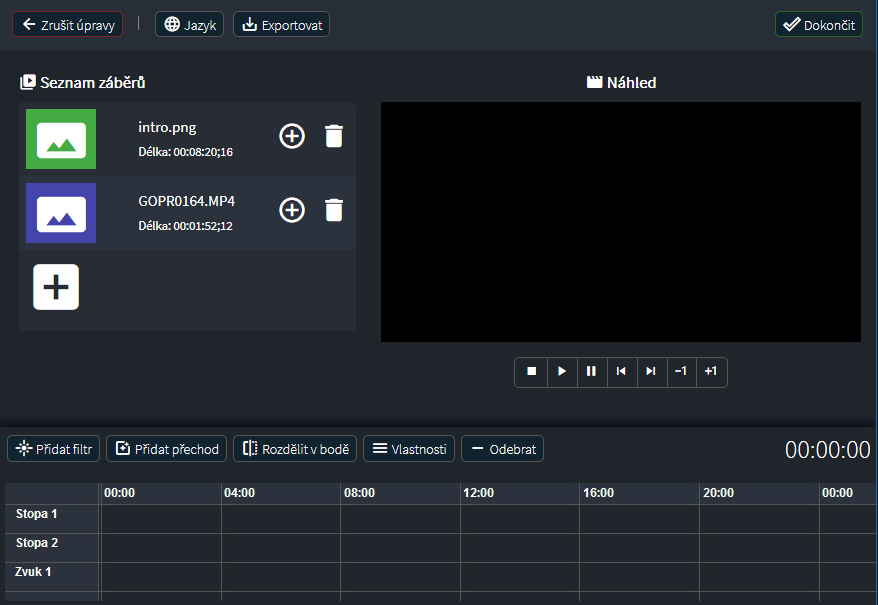
\includegraphics{obrazky-figures/mockup.png}
	}
	\caption{Prototyp uživatelského rozhraní.}\label{img:mockup}
\end{figure}
\section{Generování XML}
Se založením nového projektu je vytvořen soubor \texttt{project.mlt} obsahující hlavičku XML a odkaz na DTD schéma umístěné v repositáři projektu MLT. Poté následuje kořenový tag \texttt{<mlt>}. Uvnitř se nachází jeden playlist pro výchozí stopu \texttt{videotrack0} a hlavní kontejner \texttt{<track>} obsahující odkazy na všechny stopy v projektu. Tento hlavní kontejner musí být vždy poslední položkou v kořenovém \texttt{<mlt>}.

Uvnitř kořenového elementu se nejprve  nacházejí zdrojové soubory (elementy <producer>) u kterých jsou poznamenány následující vlastnosti -- absolutní cesta k souboru (\texttt{resource}), typ souboru (\texttt{musecut:mime\_type}), původní název souboru (\texttt{musecut:name}) a v případě video souboru délka v milisekundách (\texttt{length}). Zdrojové soubory mají id s prefixem \uv{producer} a 20 znaky náhodně generovanými při nahrávání souboru.
Po posledním elementu \texttt{<producer>} jsou pomocné playlisty
\begin{figure}[h]
	\centering
	\scalebox{0.6}{
		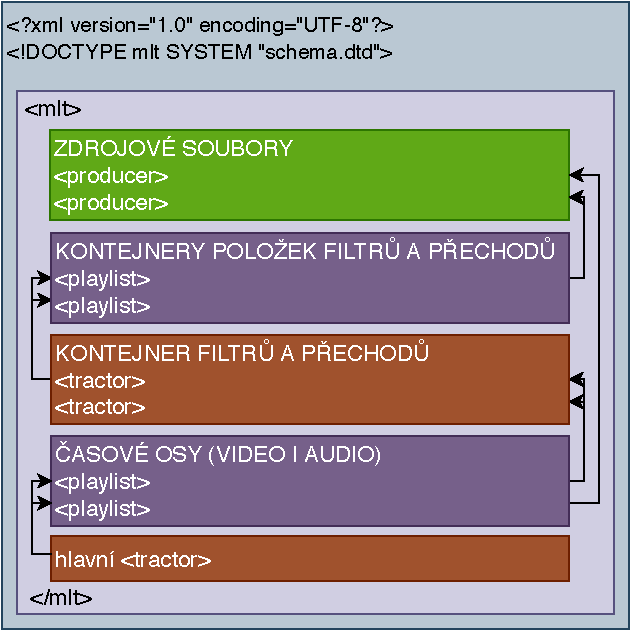
\includegraphics{obrazky-figures/schemaXML.pdf}
	}
	\caption{Obecné schména prvků generovaných souborů.}\label{img:schemaXML}
\end{figure}


\section{API serveru}
\section{Zvolené technologie}
\begin{itemize}
\item Google Material Icons -- \url{https://github.com/jossef/material-design-icons-iconfont}
\item Visual timeline -- vis.js \url{https://github.com/almende/vis}
\item FFMPEG JS API: \url{https://github.com/bilashcse/Online-Video-Editor}
\item FFmpeg v~JavaScriptu: \url{https://github.com/bgrins/videoconverter.js}
\item Python knihovna pro usnadnění práce s~MLT frameworkem: \url{https://github.com/antiboredom/vidpy}
\end{itemize}
Emaily:
\begin{itemize}
\item odesílání \texttt{nodemailer}
\item zachytávání pro testování \texttt{Papercut} / \texttt{smtp-sink} (node.js řešení)
\end{itemize}

ExpressJs (zkráceně Express) je webový framework pro Node.js. Express poskytuje knihovny užitečné pro zajištění základních funkcí webového serveru (routování, podpora šablonovacího systému pro generování stránek, zpracování dotazů, parametrů, sezení a cookies, autentifikaci, vytváření odpovědí, zpracování chyb, aj.).

Volba PHP vs Node.js. Volba EcmaScript vs TypeScript vs CoffeeScript.

\subsection{Node.js}
Node.js vytváří běhové prostředí JavaScriptu postavené na JavaScriptovém enginu V8 od firmy Google. Umožňuje používat JavaScript jako systémový jazyk, který má přístup k paměťi, bufferům, procesům, souborům a soketům. Cílem Node.js je poskytovat snadnou cestu k vytvoření škálovatelných síťových aplikací. Node.js nepoužívá vlákna, je založen na událostech a asynchronním vykonávání blokujících operací, umožňuje snadnou modularitu. Právě eliminací blokujících operací pomocí asynchronní obsluhy řízenou událostmi lze dosáhnout vysokého výkonu. PHP vytváří pro každý požadavek samostatné vlákno a v případě blokující operace čeká na vyřízení, Node.js používá pro všechny požadavky jedno vlákno a namísto paralelního zpracování používá Node.js pseudoparalelní zpracování.

Pro porovnání rychlosti vykonání programu, uvedu příklad jednoduchého programu, ve kterém se v prázdném cyklu inkrementuje miliadkrát čítač. Doba běhu programu je pro jednotlivé jazyky následující -- JavaScript (Node.js verze 9.3.0) 0,635 sekund, jazyk C (Apple LLVM 8.1.0) 2,398 sekund a Python (3.6.1) 31,096 sekund. Všechny testy probíhaly na zařízení MacBook Pro s procesorem Intel Core i7 2,8 GHz. Překladač V8 JavaScript kompiluje namísto interpretování, díky tomu lze využívat vysokoúrovňový jazyk bez nutnosti vzdát se rychlosti kompilovaných jazyků.\cite{MasteringNodejs}

JavaScript na klientské straně je pro interaktivní webovou aplikaci nutnost. Díky běhu JavaScriptu na klientské i serverové části mohou programátoři používat jeden jazyk v rámci projektu. Dále se otevírá možnost používat stejný kód na serveru i na straně klienta. Stačí vhodně členit funkce do modulů a tyto moduly poté importovat jak na straně serveru, tak na straně klienta. V mé práci takto sdílím kód pro práci s časovými značkami.

\subsubsection{Souborový systém}
Práci se souborovým systémem umožňuje modul File System (\texttt{fs}). Používání funkcí modulu \texttt{fs} je podobné POSIX funkcím jazyka C. Všechny funkce mají synchronní a asynchronní variantu. U I/O operací je silně doporučeno používat asynchronní práci se souborovým systémem. Asynchronní funkce mají jako poslední parametr callback, který se zavolá po dokončení operace. Callbacku je jako první parametr předán objekt pro uchování chyb a poté volitelně data operace. Callback je volán při úspěchu i neúspěchu, neúspěch je indikován objektem 1. parametru. Dalším modulem spojeným se souborovým systémem je \texttt{path}, který poskytuje nástroje pro práci s cestami k souborům a adresářům. Jak vypadá asynchronní čtení souboru ukazuje následující ukázka.
\begin{lstlisting}[style=JavaScript]
fs.open(path.join(projectPath, 'processing')), 'wx', (err, fd) => {
	if (err) throw err;
	// prace se souborem
	fs.close(fd, (err) => {
		if (err) console.error(err.stack);
	};
});
console.log('stale se muze cekat na nacteni souboru);
\end{lstlisting}

Funkce \texttt{fs.open} je zavolána, vytvoří požadavek souborovému systému a namísto aktivního čekání je funkce uspána a pokračuje se dál vykonáváním příkazů pod \texttt{fs.open}. V tomto případě by se vypsal do terminálu text \uv{stale se muze cekat na nacteni souboru} a k práci se souborem by se JavaScriptový engine vrátil až po zpřístupnění požadovaného souboru. Z toho plyne, že I/O operace jednoho požadavku nebrzdí vykonávání souběžných požadavků.

\subsubsection{Práce s procesy}
Díky událostem a asynchronnímu přístupu k blokujícím požadavkům není problém čekat na mnohem náročnější operace, než je práce se souborovým systémem. V projektu je potřeba zpracovávat, konvertovat a získávat informace o multimédiích. Pro JavaScript například není problém vytvořit potomka, který zpracuje videosoubor, a po skončení potomka pracovat s jeho výstupem. U PHP by to byl problém a čekající procesy by mohly způsobit vyčerpání prostředků serveru. Práci s procesy zpřístupňuje modul Child Processes (\texttt{child\_process}). Z něj využívám funkci \texttt{exec}, který vytvoří shell a umožní v něm vykonávat příkazy. Po dokončení posledního příkazu je k dispozici obsah standardního výstupu a standardního chybového výstupu. Použití příkazu \texttt{exec} demonstruje následující ukázka.
\begin{lstlisting}[style=JavaScript]
exec(`ffmpeg -i ${filepath} 2>&1 | grep Duration | cut -d \' \' -f 4 | sed s/,// | sed s/\\\\./,/`,
    (err, stdout, stderr) => {
		if (err) console.error(err);
		else {
		    console.log(stdout.trim());
	    }
});
\end{lstlisting}
Funkce \texttt{exec} vytvoří potomka a v rámci něj získá informaci o délce souboru \text{filepath}. Délku vypíše v této ukázce na obrazovku, ale pomocí Promises\footnote{Promise -- objekt, který reprezentuje budoucí úspěšné/neúspěšné dokončení asynchronní události a jeho budoucí hodnotu, \url{https://developer.mozilla.org/en-US/docs/Web/JavaScript/Reference/Global_Objects/Promise}.} je možné vytvořit funkci \texttt{getDuration} a délku asynchronně vracet.

\subsubsection{Import modulů}
Moduly zastřešují související funkce do jednoho celku. Moduly obvykle obsahují proměnné a funkce, které se zpřístupní importováním. Aby bylo možné funkce a promměnné importovat, je nutné v modulu uvádět klíčové slovo \text{export}. Pokud máme v modulu více funkcí, musíme uvést, kterou funkci chceme importovat. Při neuvedení se importuje výchozí export. Pokud chceme používat více funkcí jedním importem, je nutné v modulu veškeré funkce a proměnné obalit do společného objektu, který bude výchozí export. Následující ukázka využívá jednoho hlavního objektu, který je výchozím exportem.
\begin{lstlisting}[style=JavaScript]
export default {
	subDuration(durationA, durationB) {
		// ...
		return subResult;
	},
	addDuration(durationA, durationB) {
		// ...
		return addResult;
	},
	// ...
}
\end{lstlisting}

Pokud chceme moduly použít, je postup jak na straně serveru, tak i na straně klienta (v React) stejná.
\begin{lstlisting}[style=JavaScript]
import timeManager from '../../models/timeManager';
let actualTime = timeManager.addDuration(timeA, timeB);
\end{lstlisting}

Moduly jsou používány v rámci jednoho projektu. Pokud potřebujeme rozšířit funkcionalitu projektu a další funkce, můžeme sáhnout po balíčkovém systému \texttt{npm}.\footnote{npm -- balíčkový systém pro Node.js, \url{https://www.npmjs.com/}.} K 22. dubnu 2019 bylo v systému registrováno téměř 810 tisíc balíčků.\footnote{\url{http://www.modulecounts.com/}} Správce \texttt{npm} je výchozí balíčkový systém Node.js, jedná se obdobu správce závislostí \texttt{Composer} pro PHP.

\subsubsection{Express framework}

\subsection{TypeScript, ECMAScript}
Jedná se o programovací jazyk se syntaxí inspirovanou jazykem C, který se překládá do JavaScriptu. TypeScript je nadstavba nad JavaScriptem, program v JavaScriptu je validním programem v TypeScriptu. Přináší silnou typovou kontrolu, třídy (dnes i v ES6), rozhraní, dědičnost. Offline překlad do JavaScriptu odhalí syntaktické chyby, a volitelně zajistí kompatibilitu se standardy ES3 a ES5 (alternativou je \textit{Babel}). Dále přidává spoustu \uv{syntaktického cukru} -- gettery/settery, výčtové typy, promises. Podporuje integraci s Angular 2 i React.

Na druhou stranu je typová kontrola plnohodnotná pouze pokud všechny balíčky obsahují hlavičkové soubory TS. TypeScript je nutné začlenit do vývojového procesu s Node.js a React. Během vývoje se při každé změně zdrojového kódu musí provést kompilace do JavaScriptu. Pro začínajících programátory a pro malé projekty zavádí složitost, která nemusí převážit výhody zavedení.

S příchodem ES6 přejal standard z TypeScriptu deklaraci proměnných s platností v daném rámci bez vedlejších efektů (\texttt{let}), možnost vytvářet třídy, dědičnost, rest parametry, promises a další. Hlavní výhodou zůstává silné typování a kontrola syntaxe při kompilaci. Vzhledem k mým předchozím zkušenostem s jazykem PHP jsem tyto vlastnosti nepožadoval, proto jsem se rozhodl použít standard ES6 a novější revize. Zpětnou kompatibilitu klientského JavaScriptu jsem zajistil nástrojem \textit{Babel}.

\subsection{React}

\chapter{Realizace, experimenty}
\begin{figure}[h]
	\centering
	\scalebox{0.4}{
		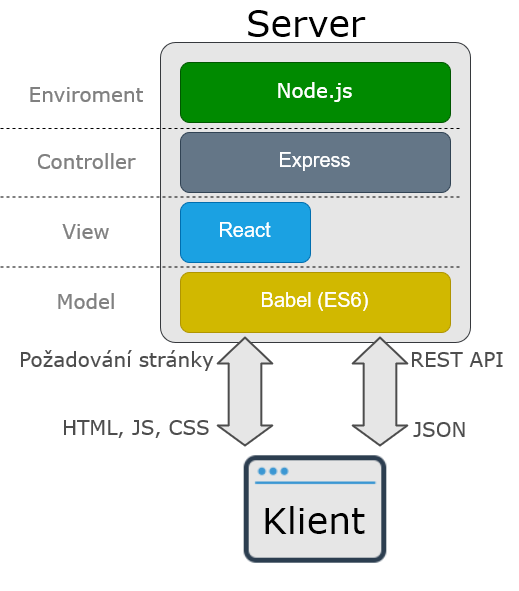
\includegraphics{obrazky-figures/server-architektura.png}
	}
	\caption{Architera serveru.}\label{img:server-architektura}
\end{figure}

\section{XML}
Výběr knihovny pro práci s XML.
Přímá práce s XML / konverze do JSON a zpět.
Způsoby přímé práce s XML: SAX / DOM.
\url{https://github.com/zeligzhou/xmldom-qsa}\\
\url{https://github.com/nfarina/xmldoc}\\
\url{https://www.npmjs.com/package/jsdom}

\section{REST API}
\url{https://scotch.io/tutorials/build-a-restful-api-using-node-and-express-4}\\
\url{https://restapitutorial.com/lessons/httpmethods.html}\\
\url{https://editor.swagger.io/}

\section{Zpracování vstupních videí}
Framework \textit{MLT} pracuje s videii po snímcích. Uživatelé videoeditorů pracují s časem na časové ose. Časové značky je nutné převádět na konkrétní snímek ve videu a naopak je nutné získat z videa celkový čas a celkový počet snímků. Spočítání snímků a celkového času videa zvládne program \texttt{ffmpeg} i \texttt{ffprobe}. Problém nastává, pokud chceme získat snímek videa v určitém čase. Získat snímek trojčlenkou ($ (pocet\ snimku / celkovy\ cas) * aktualni\ cas $) by bylo možné za předpokladu, že všechny snímky trvají shodnou dobu, tato vlastnost videí se nazývá \textit{Constatnt Frame rate (CFR)}. CFR videa mají stálou snímkovací frekvenci udávanou v hertzích (Hz) nebo snímcích za sekundu (FPS), například 60 FPS.\footnote{\url{https://en.wikipedia.org/wiki/Variable_frame_rate}} Kromě video kontejneru AVI jej popdorují všehchny rozšířené kontejnery.\footnote{\url{https://en.wikipedia.org/wiki/Comparison_of_video_container_formats}} Opakem jsou videa s promnělivou snímkovací frekvencí -- \textit{Variable Frame Rate (VFR)}.\footnote{\url{https://www.bandicam.com/support/tips/vfr-cfr/}} Promměnná snímkovací frekvence je efektivní způsob, jakým lze získat video s vysokou snímkovací frekvecí a nízkou velikostí výsledného souboru. Pokud bychom zaznamenávali obrazovku, VFR by ukládalo snímky pouze při změně na obrazovce, zatímco CFR by snímky zaznamenávalo neustále. S VFR natáčejí fotoaparáty\footnote{\url{https://camerajabber.com/variable-frame-rate-recording-video/}} i chytré telefony. VFR je tedy mnohem lepší způsob snímkování než CFV, pokud chceme video sdílet bez úprav. Úpravy VFR videí jsou problematické a například Sony Vegas jej nepodporuje, Adobe Premiere Pro VFR podporuje od ledna 2018\footnote{\url{https://www.premierebro.com/blog/premiere-pro-1201-update-variable-frame-rate-and-new-features}} a Shotcut VFR detekuje a nabídne konverzi na video s CFR\footnote{\url{https://github.com/mltframework/mlt/commit/fa4deb88ed233810d63ea8120aaa1783cc170a0e}}.

Všechny nahraná videa jsou na serveru překonvertována na videa s CFR, nejprve s nízkým rozlišení o šířce 480 px pro zobrazení náhledu v prohlížeči. Konverze probíhá do kontejneru MP4 obsahující video formátu H.264 a AAC audio. Tento formát podporuje prohlížeč Chrome, Firefox, Internet Explorer, Opera, Safari.\footnote{\url{https://developer.mozilla.org/en-US/docs/Web/HTML/Supported_media_formats#Browser_compatibility}} Po překonvertování je video zasláno spolu s délkou videa a počtem snímků zpět prohlížeči. Poté se video překonvertuje se stejnými vlastnostmi ale v původním rozlišení pro urychlení vyvádění výsledného videa. Počet snímků obou videí je shodný, náhledové video je ale získáno 4x až 5x rychleji.

\chapter{Testování}
Pro JavaScript existuje řada testovacích frameworků. Dva nejčasttěji používané jsou \textit{Jasmine}\footnote{Jasmine -- \url{jasmine.github.io}} a \textit{QUnit}\footnote{QUnit\url{http://qunitjs.com}}. Jasmin testy lze vizualozovat nástroji \textit{Testem} (CLI runner) a \textit{Protractor} (klikání v browseru). \textit{Protractor} <- \textit{Selenium}.

?? Mocha pro Node.js + Typescript ??

\subsection{Průběžná integrace (CI)}
CI (Continous integration) - build server nad všemi commity spouští testy a v případě chyb reportuje. Vhodné pro práci více vývojářů na projektu. Známými nástroji je \textit{Jenkins} a \textit{TeamCity}. Build server postupuje v následujících krocích:
\begin{enumerate}
\item kontrola na novější verzi zdrojového kódu, zvýší se číslo sestavení
\item sestaví aplikaci na serveru
\item spustí server-side unit testy
\item zabalí aplikaci pro vývoj
\item zabalenou aplikaci nainstaluje ve vývojovém prostředí
\item spustí server-side integrační testy
\item spustí JavaScriptové unit testy, integrační testy a akceptační testy
\item označí build jako splňující testy nebo jako nevyhovující v případě, že selže jeden z předchozích bodů
\item v případě, že build neprochází testy, upozorní vývojáře, který danou změnu provedl
\end{enumerate}

\subsection{Cíl testování}
\begin{itemize}
\item testování modelu
\item testování stavu aplikace
\item test vykreslování
\item testování DOM událostí
\item akceptační testy
\end{itemize}
\cite{Mastering_TypeScript}

\chapter{Závěr}
V~závěru bych rád shrnul úkony, které mě čekají v~letním semestru.

Zjistit možnosti JavaScriptu ve zpracování multimédií. Efekty nebo přechody je možné simulovat přímo v~prohlížeči.\,\cite{ManipulatingVideo} V~nadcházejícím semestru bude cílem mimo jiné zhodnotit dopad na výkon přehrávače při simulování efektů na straně prohlížeče.

Porovnat a popřemýšlet o~server/client side přístupu. Při přiložení video-souboru je nutné video předzpracovat (délka, miniatura), jsou dvě možnosti -- předzpracování provede server, uživatel musí počkat na nahrání a předzpracování souboru, nebo provede předzpracování klient, JavaScript internetového prohlížeče, výhodou je, že uživatel nemusí čekat na nahrání videa na server.

Zkusit vytvořit algoritmus pro serializaci/deserializaci projektu -- generování XML souboru na základě uživatelských akcí.

V~rámci návrhu byla vytvořena statická stránka video editoru. V~nadcházejícím semestru bude nutné napojit rozhraní na API serveru a implementovat funkčnost na straně klienta.

\section{TODO}
Našel jsem tyto předchozí práce:\\
\begin{itemize}
\item \url{https://primo.lib.vutbr.cz/primo-explore/fulldisplay?docid=420BUT_Aleph000135488&context=L&vid=420BUT&search_scope=Everything&tab=default_tab&lang=cs_CZ}
\item \url{https://primo.lib.vutbr.cz/primo-explore/fulldisplay?docid=420BUT_DSpace11012/54562&context=L&vid=420BUT&search_scope=Everything&tab=default_tab&lang=cs_CZ}
\item \url{https://primo.lib.vutbr.cz/primo-explore/fulldisplay?docid=420BUT_DSpace11012/55948&context=L&vid=420BUT&search_scope=Everything&tab=default_tab&lang=cs_CZ}
\item \url{https://primo.lib.vutbr.cz/primo-explore/fulldisplay?docid=420BUT_Aleph000135647&context=L&vid=420BUT&search_scope=Everything&tab=default_tab&lang=cs_CZ}
\end{itemize}

\begin{itemize}
\item \textbf{Podívat se na techniky základu střihu - jak udělat video, aby editor nutil udělat hezké videa
\item \textbf{umožnit přesouvání prvků s přechodem / do přechodu}
\item \textbf{controller přesunout a rozčlenit do modelů, používat promises, odchytávat chyby, systematicky vracet JSON v controlleru, viz vygenerovaný kód ze Swagger}
}
\end{itemize}

%===============================================================================
